% REV00 Tue 04 May 2021 13:55:16 WIB
% START Tue 04 May 2021 13:55:16 WIB

\chapter{A MARRIAGE CONTRACT}

There is excitement in the Veneering mansion. The mature young lady is
going to be married (powder and all) to the mature young gentleman, and
she is to be married from the Veneering house, and the Veneerings are to
give the breakfast. The Analytical, who objects as a matter of principle
to everything that occurs on the premises, necessarily objects to the
match; but his consent has been dispensed with, and a spring-van is
delivering its load of greenhouse plants at the door, in order that
to-morrow’s feast may be crowned with flowers.

The mature young lady is a lady of property. The mature young gentleman
is a gentleman of property. He invests his property. He goes, in
a condescending amateurish way, into the City, attends meetings of
Directors, and has to do with traffic in Shares. As is well known to the
wise in their generation, traffic in Shares is the one thing to have to
do with in this world. Have no antecedents, no established character, no
cultivation, no ideas, no manners; have Shares. Have Shares enough to
be on Boards of Direction in capital letters, oscillate on mysterious
business between London and Paris, and be great. Where does he come
from? Shares. Where is he going to? Shares. What are his tastes? Shares.
Has he any principles? Shares. What squeezes him into Parliament?
Shares. Perhaps he never of himself achieved success in anything, never
originated anything, never produced anything? Sufficient answer to all;
Shares. O mighty Shares! To set those blaring images so high, and to
cause us smaller vermin, as under the influence of henbane or opium, to
cry out, night and day, ‘Relieve us of our money, scatter it for us, buy
us and sell us, ruin us, only we beseech ye take rank among the powers
of the earth, and fatten on us’!

While the Loves and Graces have been preparing this torch for Hymen,
which is to be kindled to-morrow, Mr Twemlow has suffered much in his
mind. It would seem that both the mature young lady and the mature young
gentleman must indubitably be Veneering’s oldest friends. Wards of his,
perhaps? Yet that can scarcely be, for they are older than himself.
Veneering has been in their confidence throughout, and has done much to
lure them to the altar. He has mentioned to Twemlow how he said to
Mrs Veneering, ‘Anastatia, this must be a match.’ He has mentioned to
Twemlow how he regards Sophronia Akershem (the mature young lady) in the
light of a sister, and Alfred Lammle (the mature young gentleman) in the
light of a brother. Twemlow has asked him whether he went to school as
a junior with Alfred? He has answered, ‘Not exactly.’ Whether Sophronia
was adopted by his mother? He has answered, ‘Not precisely so.’
Twemlow’s hand has gone to his forehead with a lost air.

But, two or three weeks ago, Twemlow, sitting over his newspaper,
and over his dry-toast and weak tea, and over the stable-yard in Duke
Street, St James’s, received a highly-perfumed cocked-hat and monogram
from Mrs Veneering, entreating her dearest Mr T., if not particularly
engaged that day, to come like a charming soul and make a fourth at
dinner with dear Mr Podsnap, for the discussion of an interesting family
topic; the last three words doubly underlined and pointed with a note
of admiration. And Twemlow replying, ‘Not engaged, and more than
delighted,’ goes, and this takes place:

‘My dear Twemlow,’ says Veneering, ‘your ready response to Anastatia’s
unceremonious invitation is truly kind, and like an old, old friend. You
know our dear friend Podsnap?’

Twemlow ought to know the dear friend Podsnap who covered him with so
much confusion, and he says he does know him, and Podsnap reciprocates.
Apparently, Podsnap has been so wrought upon in a short time, as to
believe that he has been intimate in the house many, many, many years.
In the friendliest manner he is making himself quite at home with his
back to the fire, executing a statuette of the Colossus at Rhodes.
Twemlow has before noticed in his feeble way how soon the Veneering
guests become infected with the Veneering fiction. Not, however, that he
has the least notion of its being his own case.

‘Our friends, Alfred and Sophronia,’ pursues Veneering the veiled
prophet: ‘our friends Alfred and Sophronia, you will be glad to hear, my
dear fellows, are going to be married. As my wife and I make it a family
affair the entire direction of which we take upon ourselves, of course
our first step is to communicate the fact to our family friends.’

[‘Oh!’ thinks Twemlow, with his eyes on Podsnap, ‘then there are only
two of us, and he’s the other.’)

‘I did hope,’ Veneering goes on, ‘to have had Lady Tippins to meet you;
but she is always in request, and is unfortunately engaged.’

[‘Oh!’ thinks Twemlow, with his eyes wandering, ‘then there are three of
us, and SHE’S the other.’)

‘Mortimer Lightwood,’ resumes Veneering, ‘whom you both know, is out of
town; but he writes, in his whimsical manner, that as we ask him to be
bridegroom’s best man when the ceremony takes place, he will not refuse,
though he doesn’t see what he has to do with it.’

[‘Oh!’ thinks Twemlow, with his eyes rolling, ‘then there are four of
us, and HE’S the other.’)

‘Boots and Brewer,’ observes Veneering, ‘whom you also know, I have not
asked to-day; but I reserve them for the occasion.’

[‘Then,’ thinks Twemlow, with his eyes shut, ‘there are si--’ But here
collapses and does not completely recover until dinner is over and the
Analytical has been requested to withdraw.)

‘We now come,’ says Veneering, ‘to the point, the real point, of our
little family consultation. Sophronia, having lost both father and
mother, has no one to give her away.’

‘Give her away yourself,’ says Podsnap.

‘My dear Podsnap, no. For three reasons. Firstly, because I couldn’t
take so much upon myself when I have respected family friends to
remember. Secondly, because I am not so vain as to think that I look
the part. Thirdly, because Anastatia is a little superstitious on the
subject and feels averse to my giving away anybody until baby is old
enough to be married.’

‘What would happen if he did?’ Podsnap inquires of Mrs Veneering.

‘My dear Mr Podsnap, it’s very foolish I know, but I have an instinctive
presentiment that if Hamilton gave away anybody else first, he would
never give away baby.’ Thus Mrs Veneering; with her open hands pressed
together, and each of her eight aquiline fingers looking so very like
her one aquiline nose that the bran-new jewels on them seem necessary
for distinction’s sake.

‘But, my dear Podsnap,’ quoth Veneering, ‘there IS a tried friend of
our family who, I think and hope you will agree with me, Podsnap, is
the friend on whom this agreeable duty almost naturally devolves. That
friend,’ saying the words as if the company were about a hundred and
fifty in number, ‘is now among us. That friend is Twemlow.’

‘Certainly!’ from Podsnap.

‘That friend,’ Veneering repeats with greater firmness, ‘is our dear
good Twemlow. And I cannot sufficiently express to you, my dear Podsnap,
the pleasure I feel in having this opinion of mine and Anastatia’s so
readily confirmed by you, that other equally familiar and tried friend
who stands in the proud position--I mean who proudly stands in the
position--or I ought rather to say, who places Anastatia and myself in
the proud position of himself standing in the simple position--of baby’s
godfather.’ And, indeed, Veneering is much relieved in mind to find that
Podsnap betrays no jealousy of Twemlow’s elevation.

So, it has come to pass that the spring-van is strewing flowers on
the rosy hours and on the staircase, and that Twemlow is surveying the
ground on which he is to play his distinguished part to-morrow. He has
already been to the church, and taken note of the various impediments in
the aisle, under the auspices of an extremely dreary widow who opens the
pews, and whose left hand appears to be in a state of acute rheumatism,
but is in fact voluntarily doubled up to act as a money-box.

And now Veneering shoots out of the Study wherein he is accustomed,
when contemplative, to give his mind to the carving and gilding of
the Pilgrims going to Canterbury, in order to show Twemlow the little
flourish he has prepared for the trumpets of fashion, describing how
that on the seventeenth instant, at St James’s Church, the Reverend
Blank Blank, assisted by the Reverend Dash Dash, united in the bonds of
matrimony, Alfred Lammle Esquire, of Sackville Street, Piccadilly,
to Sophronia, only daughter of the late Horatio Akershem, Esquire,
of Yorkshire. Also how the fair bride was married from the house of
Hamilton Veneering, Esquire, of Stucconia, and was given away by Melvin
Twemlow, Esquire, of Duke Street, St James’s, second cousin to Lord
Snigsworth, of Snigsworthy Park. While perusing which composition,
Twemlow makes some opaque approach to perceiving that if the Reverend
Blank Blank and the Reverend Dash Dash fail, after this introduction, to
become enrolled in the list of Veneering’s dearest and oldest friends,
they will have none but themselves to thank for it.

After which, appears Sophronia (whom Twemlow has seen twice in his
lifetime), to thank Twemlow for counterfeiting the late Horatio Akershem
Esquire, broadly of Yorkshire. And after her, appears Alfred (whom
Twemlow has seen once in his lifetime), to do the same and to make a
pasty sort of glitter, as if he were constructed for candle-light only,
and had been let out into daylight by some grand mistake. And after
that, comes Mrs Veneering, in a pervadingly aquiline state of figure,
and with transparent little knobs on her temper, like the little
transparent knob on the bridge of her nose, ‘Worn out by worry and
excitement,’ as she tells her dear Mr Twemlow, and reluctantly revived
with curacoa by the Analytical. And after that, the bridesmaids begin
to come by rail-road from various parts of the country, and to come like
adorable recruits enlisted by a sergeant not present; for, on arriving
at the Veneering depot, they are in a barrack of strangers.

So, Twemlow goes home to Duke Street, St James’s, to take a plate of
mutton broth with a chop in it, and a look at the marriage-service, in
order that he may cut in at the right place to-morrow; and he is low,
and feels it dull over the livery stable-yard, and is distinctly aware
of a dint in his heart, made by the most adorable of the adorable
bridesmaids. For, the poor little harmless gentleman once had his fancy,
like the rest of us, and she didn’t answer (as she often does not),
and he thinks the adorable bridesmaid is like the fancy as she was then
(which she is not at all), and that if the fancy had not married some
one else for money, but had married him for love, he and she would
have been happy (which they wouldn’t have been), and that she has a
tenderness for him still (whereas her toughness is a proverb). Brooding
over the fire, with his dried little head in his dried little hands,
and his dried little elbows on his dried little knees, Twemlow is
melancholy. ‘No Adorable to bear me company here!’ thinks he. ‘No
Adorable at the club! A waste, a waste, a waste, my Twemlow!’ And so
drops asleep, and has galvanic starts all over him.

Betimes next morning, that horrible old Lady Tippins (relict of the late
Sir Thomas Tippins, knighted in mistake for somebody else by His
Majesty King George the Third, who, while performing the ceremony, was
graciously pleased to observe, ‘What, what, what? Who, who, who?
Why, why, why?’) begins to be dyed and varnished for the interesting
occasion. She has a reputation for giving smart accounts of things, and
she must be at these people’s early, my dear, to lose nothing of the
fun. Whereabout in the bonnet and drapery announced by her name, any
fragment of the real woman may be concealed, is perhaps known to her
maid; but you could easily buy all you see of her, in Bond Street; or
you might scalp her, and peel her, and scrape her, and make two Lady
Tippinses out of her, and yet not penetrate to the genuine article. She
has a large gold eye-glass, has Lady Tippins, to survey the proceedings
with. If she had one in each eye, it might keep that other drooping
lid up, and look more uniform. But perennial youth is in her artificial
flowers, and her list of lovers is full.

‘Mortimer, you wretch,’ says Lady Tippins, turning the eyeglass about
and about, ‘where is your charge, the bridegroom?’

‘Give you my honour,’ returns Mortimer, ‘I don’t know, and I don’t
care.’

‘Miserable! Is that the way you do your duty?’

‘Beyond an impression that he is to sit upon my knee and be seconded
at some point of the solemnities, like a principal at a prizefight, I
assure you I have no notion what my duty is,’ returns Mortimer.

Eugene is also in attendance, with a pervading air upon him of having
presupposed the ceremony to be a funeral, and of being disappointed. The
scene is the Vestry-room of St James’s Church, with a number of leathery
old registers on shelves, that might be bound in Lady Tippinses.

But, hark! A carriage at the gate, and Mortimer’s man arrives, looking
rather like a spurious Mephistopheles and an unacknowledged member
of that gentleman’s family. Whom Lady Tippins, surveying through her
eye-glass, considers a fine man, and quite a catch; and of whom Mortimer
remarks, in the lowest spirits, as he approaches, ‘I believe this is my
fellow, confound him!’ More carriages at the gate, and lo the rest of
the characters. Whom Lady Tippins, standing on a cushion, surveying
through the eye-glass, thus checks off. ‘Bride; five-and-forty if a
day, thirty shillings a yard, veil fifteen pound, pocket-handkerchief
a present. Bridesmaids; kept down for fear of outshining bride,
consequently not girls, twelve and sixpence a yard, Veneering’s flowers,
snub-nosed one rather pretty but too conscious of her stockings, bonnets
three pound ten. Twemlow; blessed release for the dear man if she really
was his daughter, nervous even under the pretence that she is, well he
may be. Mrs Veneering; never saw such velvet, say two thousand pounds
as she stands, absolute jeweller’s window, father must have been a
pawnbroker, or how could these people do it? Attendant unknowns; pokey.’

Ceremony performed, register signed, Lady Tippins escorted out of sacred
edifice by Veneering, carriages rolling back to Stucconia, servants
with favours and flowers, Veneering’s house reached, drawing-rooms most
magnificent. Here, the Podsnaps await the happy party; Mr Podsnap, with
his hair-brushes made the most of; that imperial rocking-horse, Mrs
Podsnap, majestically skittish. Here, too, are Boots and Brewer, and
the two other Buffers; each Buffer with a flower in his button-hole, his
hair curled, and his gloves buttoned on tight, apparently come prepared,
if anything had happened to the bridegroom, to be married instantly.
Here, too, the bride’s aunt and next relation; a widowed female of
a Medusa sort, in a stoney cap, glaring petrifaction at her
fellow-creatures. Here, too, the bride’s trustee; an oilcake-fed style
of business-gentleman with mooney spectacles, and an object of much
interest. Veneering launching himself upon this trustee as his oldest
friend (which makes seven, Twemlow thought), and confidentially retiring
with him into the conservatory, it is understood that Veneering is his
co-trustee, and that they are arranging about the fortune. Buffers are
even overheard to whisper Thir-ty Thou-sand Pou-nds! with a smack and a
relish suggestive of the very finest oysters. Pokey unknowns, amazed
to find how intimately they know Veneering, pluck up spirit, fold
their arms, and begin to contradict him before breakfast. What time Mrs
Veneering, carrying baby dressed as a bridesmaid, flits about among
the company, emitting flashes of many-coloured lightning from diamonds,
emeralds, and rubies.

The Analytical, in course of time achieving what he feels to be due to
himself in bringing to a dignified conclusion several quarrels he has on
hand with the pastrycook’s men, announces breakfast. Dining-room no less
magnificent than drawing-room; tables superb; all the camels out, and
all laden. Splendid cake, covered with Cupids, silver, and true-lovers’
knots. Splendid bracelet, produced by Veneering before going down, and
clasped upon the arm of bride. Yet nobody seems to think much more of
the Veneerings than if they were a tolerable landlord and landlady
doing the thing in the way of business at so much a head. The bride and
bridegroom talk and laugh apart, as has always been their manner;
and the Buffers work their way through the dishes with systematic
perseverance, as has always been THEIR manner; and the pokey unknowns
are exceedingly benevolent to one another in invitations to take
glasses of champagne; but Mrs Podsnap, arching her mane and rocking her
grandest, has a far more deferential audience than Mrs Veneering; and
Podsnap all but does the honours.

Another dismal circumstance is, that Veneering, having the captivating
Tippins on one side of him and the bride’s aunt on the other, finds
it immensely difficult to keep the peace. For, Medusa, besides
unmistakingly glaring petrifaction at the fascinating Tippins, follows
every lively remark made by that dear creature, with an audible snort:
which may be referable to a chronic cold in the head, but may also be
referable to indignation and contempt. And this snort being regular in
its reproduction, at length comes to be expected by the company, who
make embarrassing pauses when it is falling due, and by waiting for it,
render it more emphatic when it comes. The stoney aunt has likewise an
injurious way of rejecting all dishes whereof Lady Tippins partakes:
saying aloud when they are proffered to her, ‘No, no, no, not for me.
Take it away!’ As with a set purpose of implying a misgiving that if
nourished upon similar meats, she might come to be like that charmer,
which would be a fatal consummation. Aware of her enemy, Lady Tippins
tries a youthful sally or two, and tries the eye-glass; but, from the
impenetrable cap and snorting armour of the stoney aunt all weapons
rebound powerless.

Another objectionable circumstance is, that the pokey unknowns support
each other in being unimpressible. They persist in not being frightened
by the gold and silver camels, and they are banded together to defy
the elaborately chased ice-pails. They even seem to unite in some vague
utterance of the sentiment that the landlord and landlady will make a
pretty good profit out of this, and they almost carry themselves
like customers. Nor is there compensating influence in the adorable
bridesmaids; for, having very little interest in the bride, and none
at all in one another, those lovely beings become, each one of her own
account, depreciatingly contemplative of the millinery present; while
the bridegroom’s man, exhausted, in the back of his chair, appears to be
improving the occasion by penitentially contemplating all the wrong he
has ever done; the difference between him and his friend Eugene, being,
that the latter, in the back of HIS chair, appears to be contemplating
all the wrong he would like to do--particularly to the present company.

In which state of affairs, the usual ceremonies rather droop and flag,
and the splendid cake when cut by the fair hand of the bride has but
an indigestible appearance. However, all the things indispensable to
be said are said, and all the things indispensable to be done are
done (including Lady Tippins’s yawning, falling asleep, and waking
insensible), and there is hurried preparation for the nuptial journey
to the Isle of Wight, and the outer air teems with brass bands and
spectators. In full sight of whom, the malignant star of the Analytical
has pre-ordained that pain and ridicule shall befall him. For he,
standing on the doorsteps to grace the departure, is suddenly caught a
most prodigious thump on the side of his head with a heavy shoe, which
a Buffer in the hall, champagne-flushed and wild of aim, has borrowed on
the spur of the moment from the pastrycook’s porter, to cast after the
departing pair as an auspicious omen.

So they all go up again into the gorgeous drawing-rooms--all of them
flushed with breakfast, as having taken scarlatina sociably--and there
the combined unknowns do malignant things with their legs to ottomans,
and take as much as possible out of the splendid furniture. And so, Lady
Tippins, quite undetermined whether today is the day before yesterday,
or the day after to-morrow, or the week after next, fades away; and
Mortimer Lightwood and Eugene fade away, and Twemlow fades away, and
the stoney aunt goes away--she declines to fade, proving rock to the
last--and even the unknowns are slowly strained off, and it is all over.

All over, that is to say, for the time being. But, there is another time
to come, and it comes in about a fortnight, and it comes to Mr and Mrs
Lammle on the sands at Shanklin, in the Isle of Wight.

Mr and Mrs Lammle have walked for some time on the Shanklin sands, and
one may see by their footprints that they have not walked arm in arm,
and that they have not walked in a straight track, and that they have
walked in a moody humour; for, the lady has prodded little spirting
holes in the damp sand before her with her parasol, and the gentleman
has trailed his stick after him. As if he were of the Mephistopheles
family indeed, and had walked with a drooping tail.

‘Do you mean to tell me, then, Sophronia--’

Thus he begins after a long silence, when Sophronia flashes fiercely,
and turns upon him.

‘Don’t put it upon ME, sir. I ask you, do YOU mean to tell me?’

Mr Lammle falls silent again, and they walk as before. Mrs Lammle opens
her nostrils and bites her under-lip; Mr Lammle takes his gingerous
whiskers in his left hand, and, bringing them together, frowns furtively
at his beloved, out of a thick gingerous bush.

‘Do I mean to say!’ Mrs Lammle after a time repeats, with indignation.
‘Putting it on me! The unmanly disingenuousness!’

Mr Lammle stops, releases his whiskers, and looks at her. ‘The what?’

Mrs Lammle haughtily replies, without stopping, and without looking
back. ‘The meanness.’

He is at her side again in a pace or two, and he retorts, ‘That is not
what you said. You said disingenuousness.’

‘What if I did?’

‘There is no “if” in the case. You did.’

‘I did, then. And what of it?’

‘What of it?’ says Mr Lammle. ‘Have you the face to utter the word to
me?’

‘The face, too!’ replied Mrs Lammle, staring at him with cold scorn.
‘Pray, how dare you, sir, utter the word to me?’

‘I never did.’

As this happens to be true, Mrs Lammle is thrown on the feminine
resource of saying, ‘I don’t care what you uttered or did not utter.’

After a little more walking and a little more silence, Mr Lammle breaks
the latter.

‘You shall proceed in your own way. You claim a right to ask me do I
mean to tell you. Do I mean to tell you what?’

‘That you are a man of property?’

‘No.’

‘Then you married me on false pretences?’

‘So be it. Next comes what you mean to say. Do you mean to say you are a
woman of property?’

‘No.’

‘Then you married me on false pretences.’

‘If you were so dull a fortune-hunter that you deceived yourself, or
if you were so greedy and grasping that you were over-willing to be
deceived by appearances, is it my fault, you adventurer?’ the lady
demands, with great asperity.

‘I asked Veneering, and he told me you were rich.’

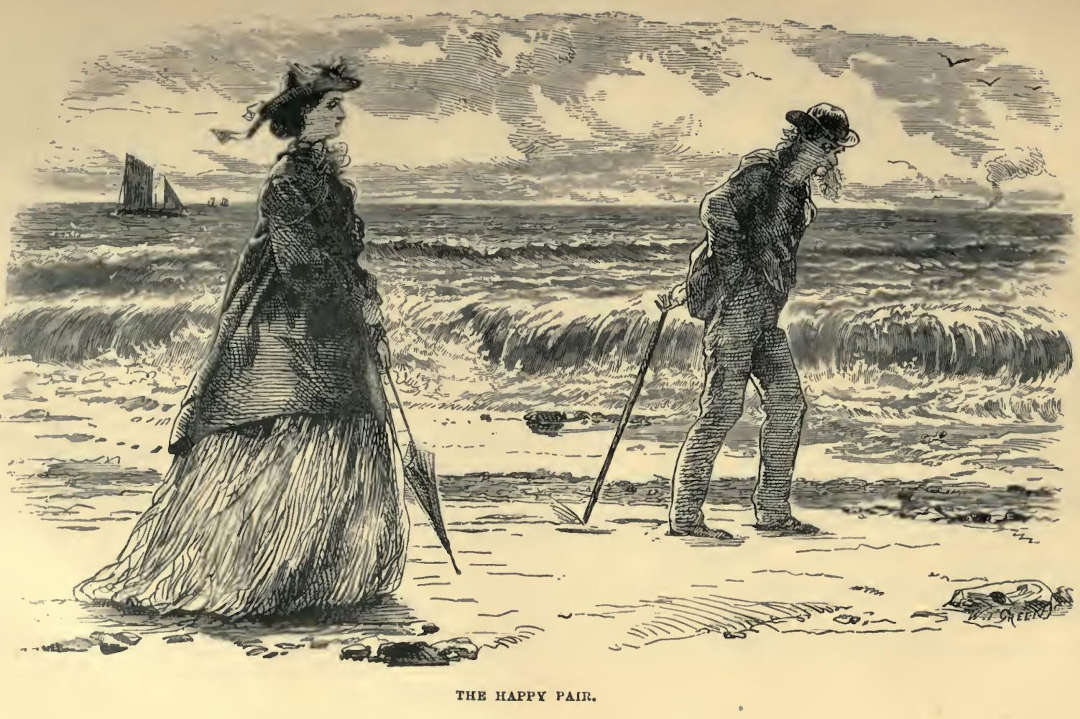
\includegraphics[scale=2.3]{01-10-01}

‘Veneering!’ with great contempt.’ And what does Veneering know about
me!’

‘Was he not your trustee?’

‘No. I have no trustee, but the one you saw on the day when you
fraudulently married me. And his trust is not a very difficult one, for
it is only an annuity of a hundred and fifteen pounds. I think there are
some odd shillings or pence, if you are very particular.’

Mr Lammle bestows a by no means loving look upon the partner of his joys
and sorrows, and he mutters something; but checks himself.

‘Question for question. It is my turn again, Mrs Lammle. What made you
suppose me a man of property?’

‘You made me suppose you so. Perhaps you will deny that you always
presented yourself to me in that character?’

‘But you asked somebody, too. Come, Mrs Lammle, admission for admission.
You asked somebody?’

‘I asked Veneering.’

‘And Veneering knew as much of me as he knew of you, or as anybody knows
of him.’

After more silent walking, the bride stops short, to say in a passionate
manner:

‘I never will forgive the Veneerings for this!’

‘Neither will I,’ returns the bridegroom.

With that, they walk again; she, making those angry spirts in the sand;
he, dragging that dejected tail. The tide is low, and seems to have
thrown them together high on the bare shore. A gull comes sweeping by
their heads and flouts them. There was a golden surface on the brown
cliffs but now, and behold they are only damp earth. A taunting roar
comes from the sea, and the far-out rollers mount upon one another,
to look at the entrapped impostors, and to join in impish and exultant
gambols.

‘Do you pretend to believe,’ Mrs Lammle resumes, sternly, ‘when you talk
of my marrying you for worldly advantages, that it was within the bounds
of reasonable probability that I would have married you for yourself?’

‘Again there are two sides to the question, Mrs Lammle. What do you
pretend to believe?’

‘So you first deceive me and then insult me!’ cries the lady, with a
heaving bosom.

‘Not at all. I have originated nothing. The double-edged question was
yours.’

‘Was mine!’ the bride repeats, and her parasol breaks in her angry hand.

His colour has turned to a livid white, and ominous marks have come to
light about his nose, as if the finger of the very devil himself had,
within the last few moments, touched it here and there. But he has
repressive power, and she has none.

‘Throw it away,’ he coolly recommends as to the parasol; ‘you have made
it useless; you look ridiculous with it.’

Whereupon she calls him in her rage, ‘A deliberate villain,’ and so
casts the broken thing from her as that it strikes him in falling. The
finger-marks are something whiter for the instant, but he walks on at
her side.

She bursts into tears, declaring herself the wretchedest, the most
deceived, the worst-used, of women. Then she says that if she had
the courage to kill herself, she would do it. Then she calls him vile
impostor. Then she asks him, why, in the disappointment of his base
speculation, he does not take her life with his own hand, under the
present favourable circumstances. Then she cries again. Then she is
enraged again, and makes some mention of swindlers. Finally, she sits
down crying on a block of stone, and is in all the known and unknown
humours of her sex at once. Pending her changes, those aforesaid marks
in his face have come and gone, now here now there, like white steps
of a pipe on which the diabolical performer has played a tune. Also his
livid lips are parted at last, as if he were breathless with running.
Yet he is not.

‘Now, get up, Mrs Lammle, and let us speak reasonably.’

She sits upon her stone, and takes no heed of him.

‘Get up, I tell you.’

Raising her head, she looks contemptuously in his face, and repeats,
‘You tell me! Tell me, forsooth!’

She affects not to know that his eyes are fastened on her as she droops
her head again; but her whole figure reveals that she knows it uneasily.

‘Enough of this. Come! Do you hear? Get up.’

Yielding to his hand, she rises, and they walk again; but this time with
their faces turned towards their place of residence.

‘Mrs Lammle, we have both been deceiving, and we have both been
deceived. We have both been biting, and we have both been bitten. In a
nut-shell, there’s the state of the case.’

‘You sought me out--’

‘Tut! Let us have done with that. WE know very well how it was. Why
should you and I talk about it, when you and I can’t disguise it? To
proceed. I am disappointed and cut a poor figure.’

‘Am I no one?’

‘Some one--and I was coming to you, if you had waited a moment. You,
too, are disappointed and cut a poor figure.’

‘An injured figure!’

‘You are now cool enough, Sophronia, to see that you can’t be injured
without my being equally injured; and that therefore the mere word is
not to the purpose. When I look back, I wonder how I can have been such
a fool as to take you to so great an extent upon trust.’

‘And when I look back--’ the bride cries, interrupting.

‘And when you look back, you wonder how you can have been--you’ll excuse
the word?’

‘Most certainly, with so much reason.

‘--Such a fool as to take ME to so great an extent upon trust. But the
folly is committed on both sides. I cannot get rid of you; you cannot
get rid of me. What follows?’

‘Shame and misery,’ the bride bitterly replies.

‘I don’t know. A mutual understanding follows, and I think it may carry
us through. Here I split my discourse (give me your arm, Sophronia),
into three heads, to make it shorter and plainer. Firstly, it’s enough
to have been done, without the mortification of being known to have been
done. So we agree to keep the fact to ourselves. You agree?’

‘If it is possible, I do.’

‘Possible! We have pretended well enough to one another. Can’t we,
united, pretend to the world? Agreed. Secondly, we owe the Veneerings
a grudge, and we owe all other people the grudge of wishing them to be
taken in, as we ourselves have been taken in. Agreed?’

‘Yes. Agreed.’

‘We come smoothly to thirdly. You have called me an adventurer,
Sophronia. So I am. In plain uncomplimentary English, so I am. So are
you, my dear. So are many people. We agree to keep our own secret, and
to work together in furtherance of our own schemes.’

‘What schemes?’

‘Any scheme that will bring us money. By our own schemes, I mean our
joint interest. Agreed?’

She answers, after a little hesitation, ‘I suppose so. Agreed.’

‘Carried at once, you see! Now, Sophronia, only half a dozen words more.
We know one another perfectly. Don’t be tempted into twitting me with
the past knowledge that you have of me, because it is identical with
the past knowledge that I have of you, and in twitting me, you
twit yourself, and I don’t want to hear you do it. With this good
understanding established between us, it is better never done. To wind
up all:--You have shown temper today, Sophronia. Don’t be betrayed into
doing so again, because I have a Devil of a temper myself.’

So, the happy pair, with this hopeful marriage contract thus signed,
sealed, and delivered, repair homeward. If, when those infernal
finger-marks were on the white and breathless countenance of Alfred
Lammle, Esquire, they denoted that he conceived the purpose of subduing
his dear wife Mrs Alfred Lammle, by at once divesting her of any
lingering reality or pretence of self-respect, the purpose would seem
to have been presently executed. The mature young lady has mighty little
need of powder, now, for her downcast face, as he escorts her in the
light of the setting sun to their abode of bliss.



